\newpage
\section{Ranking}
To answer research question 3: \textit{Is it possible to generate a ranking of tools according to their performance on unseen datasets?}; the estimators from the previous section will be used to give an estimated ranking for best strategies that could be used on that dataset. In the following section, the results will be based on the ranking generated by the F1-score estimators from the previous section. Only the NDCG based on the F1-score will be used to give the qualitative evaluation. For each experiment, the best strategy ranking estimator (either the combined F1-estimator or direct F1-estimator) will be shown and evaluated. In the last section, overall performance over all rankings will be compared to the baseline method to quantitatively evaluate the results.

\subsection{Best tool ranking}
For finding the best tool, the strategy ranking with only a single configuration per tool was created. Like stated in \autoref{sec:toolranking}, there were 2 ways of scoring this ranking. 

\subsubsection{Strategy-based scoring}
The first way of scoring was strategy-based scoring. For this experiment the direct F1 estimator was the best performing underlying estimator for generating the ranking. In figure \autoref{fig:ndcg_per_strategy}, the NDCG scores are shown with relevance according to the suggested specific strategy.
As can be seen in the figure, for two out of the fourteen datasets, the score is less than half the top score (1). This implies that for those datasets, the suggested strategy ranking placed less performing strategies higher at the top and/or gave less performing configurations of a tool priority over a better configuration. 

\begin{figure}[H]
    \centering
    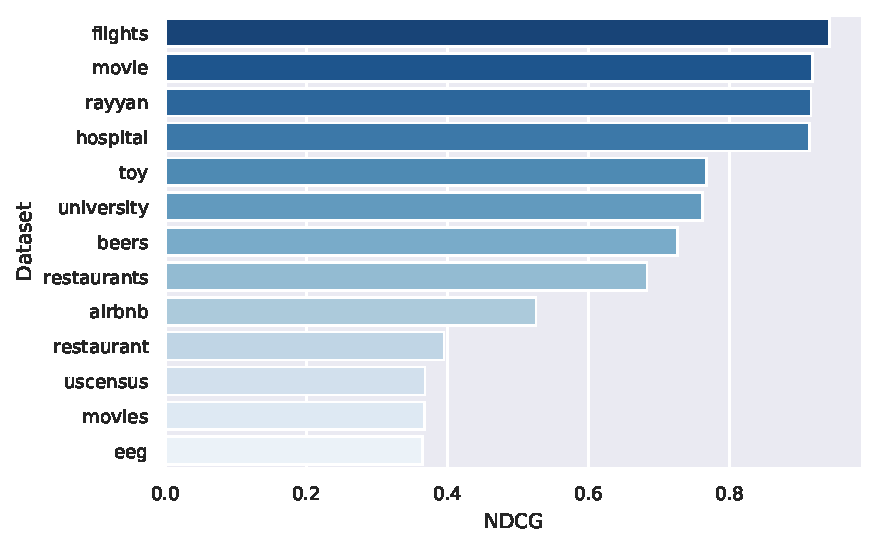
\includegraphics[width=0.7\textwidth]{thesis/Figures/RQ3/15_ranking_ndcg_combined_f1.pdf}
    \caption{NDCG per dataset for strategy ranking of the combined F1 estimator}
    \label{fig:ndcg_per_strategy}
\end{figure}


\subsubsection{Tool-based scoring}
The other way of scoring, tool-wise scoring, was were the NDCG scores calculated with relevance according to the highest scoring strategy of that tool. In this scoring way, the configurations of the ranking are disregarded and there is only a focus on the ordering of tools. The results can be seen in \autoref{fig:ndcg_per_tool}. The resulting NDCG scores are 0.27 higher than the NDCG scores for the strategy-wise scoring. This means that the recommended strategy ranking is better at finding the right tool, but not necessarily selects the best single configuration for that tool. 

\begin{figure}[H]
    \centering
    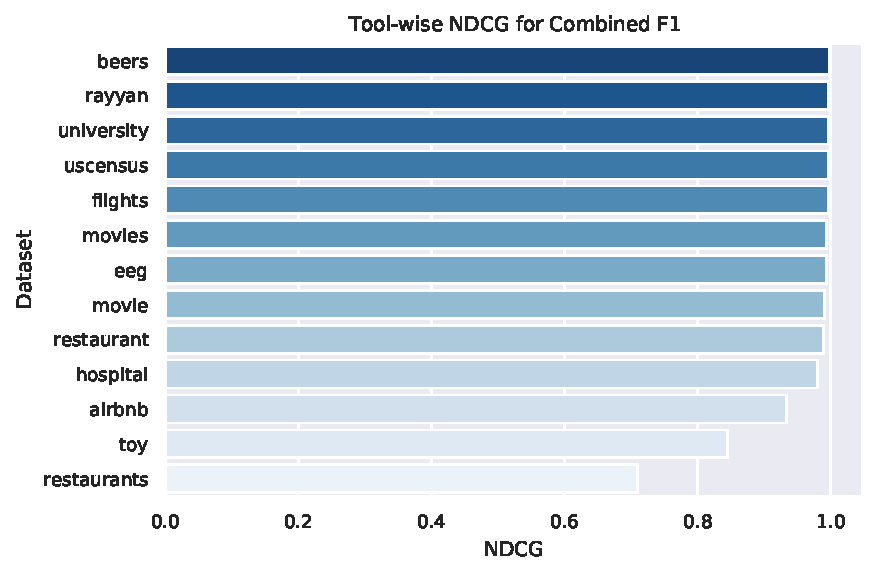
\includegraphics[width=0.7\textwidth]{thesis/Figures/RQ3/15_ranking_ndcg_combined_f1_tool_wise.pdf}
    \caption{NDCG per dataset for tool ranking of the combined F1 estimator}
    \label{fig:ndcg_per_tool}
\end{figure}


\subsection{Best configuration ranking}
Following the results from \autoref{fig:ndcg_per_tool}, where has been shown that a good ranking of tools can be made, the next section will discuss configuration ranking for a single tool. The two error detection tools that will be covered are Raha and dBoost. The two tools are the best performing tools overall and have both have numerous configuration options, making it worthwhile to generate a configuration ranking.

\paragraph{Raha} With an mean NDCG of 0.80, the configuration ranking for Raha is really promising. For most of the datasets, the ranking is near optimal. As shown in \autoref{fig:ndcg_per_config_Raha}, only for 2 datasets, the score is below half optimal. This means that for those datasets, wrong suggestions will be made for the configurations to use. For the majority of datasets, the ranking system is able to output the configuration in a ordering where the top suggestions also correspond with high performance results from the empirical study. 

\begin{figure}[H]
    \centering
    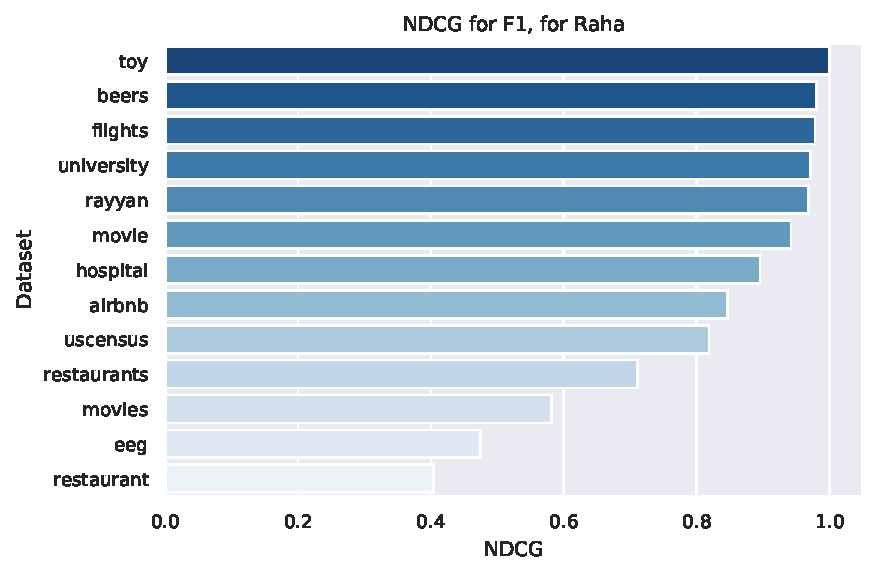
\includegraphics[width=0.8\textwidth]{thesis/Figures/RQ3/15_combined_profiler_NDCG_Raha.pdf}
    \caption{NDCG per dataset for configuration ranking of the combined F1 estimator for Raha}
    \label{fig:ndcg_per_config_Raha}
\end{figure}

\paragraph{dBoost} With an mean NDCG of 0.59, the configuration ranking for dBoost is worse than . A score of 0.59 corresponds to an just above decent ranking on average. This means that for some datasets it is able to output correct rankings, but for others it is completely not. With dBoost, the difference between the best and worst performing strategies are greater than the difference between Raha strategies. 

Also, certain dBoost configurations are locally non-sensitive, meaning that small changes in the configurations do not have a great impact on the results. These locally insensitive configurations can be grouped together based on more influential parameters. This also implies that, if an estimate for a configuration will be given, the configuration that are in the same group will also have similar estimates. If one of these estimates is an over-estimation, multiple estimations will be too high, resulting a worse ranking. Future improvements of the ranking system could include protection against these grouped estimations causing worse results.

\begin{figure}[H]
    \centering
    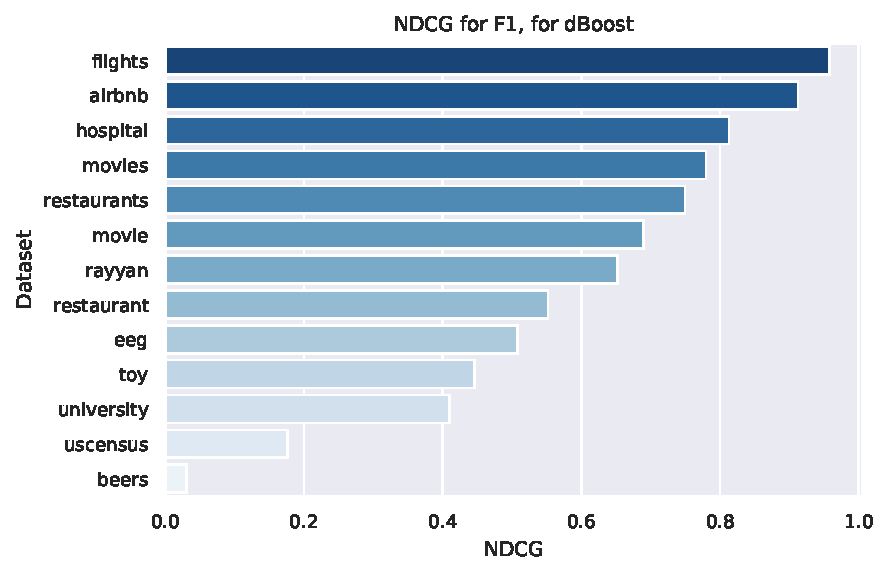
\includegraphics[width=0.8\textwidth]{thesis/Figures/RQ3/15_combined_profiler_NDCG_dBoost.pdf}
    \caption{NDCG per dataset for configuration ranking of the combined F1 estimator for dBoost}
    \label{fig:ndcg_per_config_dBoost}
\end{figure}


\subsection{Evaluation}

\begin{table}[h]
\centering
\caption{Mean NDCG comparison for tool ranking}
\begin{tabular}{lrrr}
\toprule
{} &  Baseline &       Estimator  &  Improvement \\
Metric      & Mean NDCG  &         Mean NDCG  &              \\
\midrule
Combined F1 &       0.95 &  \textbf{0.96} &     0.002 \\
F1          &       \textbf{0.96} &  0.96 &    -0.002 \\
Precision   &       \textbf{0.94} &  0.94 &    -0.000 \\
Recall      &       0.96 &  \textbf{0.97} &     0.009 \\
\bottomrule
\end{tabular}
\end{table}


\begin{table}[h]
\centering
\caption{Mean NDCG comparison for strategy ranking}
\begin{tabular}{lrrr}
\toprule
{} &  Baseline &       Estimator  &  Improvement \\
Metric      & Mean NDCG  &         Mean NDCG  &              \\
\midrule
Combined F1 &       0.54 &  \textbf{0.63} &     0.086 \\
F1          &       0.69 &  \textbf{0.75} &     0.055 \\
Precision   &       0.49 &  \textbf{0.58} &     0.090 \\
Recall      &       0.88 &  \textbf{0.90} &     0.020 \\
\bottomrule
\end{tabular}
\end{table}